\documentclass{ximera}

\begin{document}
	\author{Stitz-Zeager}
	\xmtitle{TITLE}
\mfpicnumber{1} \opengraphsfile{ExercisesforApplicationsofExponentialandLogarithmicFunctions} % mfpic settings added 


\label{ExercisesforApplicationsofExponentialandLogarithmicFunctions}

For each of the scenarios given in Exercises \ref{basicinterestexfirst} - \ref{basicinterestexlast}, 

\begin{itemize}

\item  Find the amount $A$ in the account as a function of the term of the investment $t$ in years. 

\item  To the nearest cent, determine how much is in the account after $5$, $10$, $30$ and $35$ years.  

\item  To the nearest year, determine how long will it take for the initial investment to double.  

\item  Find and interpret the average rate of change of the amount in the account from the end of
the fourth year to the end of the fifth year, and from the end of the thirty-fourth year to the
end of the thirty-fifth year.  Round your answer to two decimal places.

\end{itemize} 

\begin{enumerate}

\item  $\$500$ is invested in an account which offers $0.75 \%$, compounded monthly. \label{basicinterestexfirst}

\item  $\$500$ is invested in an account which offers $0.75 \%$, compounded continuously.

\item  $\$1000$ is invested in an account which offers $1.25 \%$, compounded monthly.

\item  $\$1000$ is invested in an account which offers $1.25 \%$, compounded continuously.

\item  $\$5000$ is invested in an account which offers $2.125 \%$, compounded monthly.

\item  $\$5000$ is invested in an account which offers $2.125 \%$, compounded continuously. \label{basicinterestexlast}

\setcounter{HW}{\value{enumi}}
\end{enumerate}

\begin{enumerate}
\setcounter{enumi}{\value{HW}}

\item  Look back at your answers to Exercises \ref{basicinterestexfirst} - \ref{basicinterestexlast}. What can be said about the difference between monthly compounding and continuously compounding the interest in those situations?  With the help of your classmates, discuss scenarios where the difference between monthly  and continuously compounded interest would be more dramatic.  Try varying the interest rate, the term of the investment and the principal.  Use computations to support your answer.

\item  How much money needs to be invested now to obtain $\$2000$ in 3 years if the interest rate in a savings account is $0.25 \%$, compounded continuously?  Round your answer to the nearest cent.

\item  How much money needs to be invested now to obtain $\$5000$ in  10 years if the interest rate in a CD is $2.25 \%$, compounded monthly?  Round your answer to the nearest cent.


\item On May, 31, 2009, the Annual Percentage Rate listed at Jeff's bank for regular savings accounts was $0.25\%$ compounded monthly.  Use Equation \ref{compoundinterest} to answer the following.

\begin{enumerate}

\item If $P = 2000$ what is $A(8)$?
\item Solve the equation $A(t) = 4000$ for $t$.
\item What principal $P$ should be invested so that the account balance is \$2000 is three years?

\end{enumerate}

\pagebreak

\item Jeff's bank also offers a 36-month Certificate of Deposit (CD) with an APR of $2.25\%$.

\begin{enumerate}

\item If $P = 2000$ what is $A(8)$?
\item Solve the equation $A(t) = 4000$ for $t$.
\item What principal $P$ should be invested so that the account balance is \$2000 in three years?
\item The Annual Percentage Yield is the \underline{simple} interest rate that returns the same amount of interest after one year as the compound interest does.  With the help of your classmates, compute the APY for this investment.

\end{enumerate}


\item  A finance company offers a promotion on $\$5000$ loans.  The borrower does not have to make any payments for the first three years, however interest will continue to be charged to the loan at $29.9 \%$ compounded continuously.  What amount will be due at the end of the three year period, assuming no payments are made?  If the promotion is extended an additional three years, and no payments are made, what amount would be due?

\item Use Equation \ref{compoundinterest} to show that the time it takes for an investment to double in value does \underline{not} depend on the principal $P$, but rather, depends only on the APR and the number of compoundings per year.  Let $n = 12$ and with the help of your classmates compute the doubling time for a variety of rates $r$.  Then look up the Rule of 72 and compare your answers to what that rule says.  If you're really interested\footnote{Awesome pun!} in Financial Mathematics, you could also compare and contrast the Rule of 72 with the Rule of 70 and the Rule of 69.

\setcounter{HW}{\value{enumi}}
\end{enumerate}

In Exercises \ref{radioactivefirst} - \ref{radioactivelast},  we list some radioactive isotopes and their associated half-lives.  Assume that each decays according to the formula $A(t) = A_{\text{\tiny $0$}}e^{kt}$ where $A_{\text{\tiny $0$}}$ is the initial amount of the material and $k$ is the decay constant. For each isotope:

\begin{itemize}

\item  Find the decay constant $k$.  Round your answer to four decimal places.

\item  Find a function which gives the amount of isotope $A$ which remains after time $t$.  (Keep the units of $A$ and $t$ the same as the given data.)

\item  Determine how long it takes for $90 \%$ of the material to decay.  Round your answer to two decimal places.  (HINT:  If $90 \%$ of the material decays, how much is left?)

\end{itemize}

\begin{enumerate}
\setcounter{enumi}{\value{HW}}

\item  Cobalt 60, used in food irradiation, initial amount 50 grams, half-life of $5.27$ years.  \label{radioactivefirst}

\item  Phosphorus 32, used in agriculture, initial amount 2 milligrams, half-life $14$ days.

\item  Chromium 51, used to track red blood cells, initial amount 75 milligrams, half-life  $27.7$ days.

\item  Americium 241, used in smoke detectors, initial amount 0.29 micrograms, half-life $432.7$ years.

\item  Uranium 235, used for nuclear power, initial amount $1$ kg, half-life  $704$ million years. \label{radioactivelast}

\setcounter{HW}{\value{enumi}}
\end{enumerate}

\begin{enumerate}
\setcounter{enumi}{\value{HW}}

\item With the help of your classmates, show that the time it takes for $90 \%$ of each isotope listed in Exercises \ref{radioactivefirst} - \ref{radioactivelast} to decay does not depend on the initial amount of the substance, but rather, on only the decay constant $k$. Find a formula, in terms of $k$ only, to determine how long it takes for $90 \%$ of a radioactive isotope to decay. 


\item In Example \ref{cardepreciationex} in Section \ref{ExponentialFunctions}, the exponential function $V(x) = 25 \left(\frac{4}{5}\right)^{x}$ was used to model the value of a car over time.  Use a change of base formula to rewrite the model in the form $V(t) = 25e^{kt}$.

\item  The Gross Domestic Product (GDP) of the US (in billions of dollars) $t$ years after the year 2000 can be modeled by: \[ G(t) = 9743.77 e^{0.0514t}\]

\begin{enumerate}

\item  Find and interpret $G(0)$.

\item  According to the model, what should have been the GDP in 2007?  In 2010?  (According to the   \href{http://1.usa.gov/iimT40}{\underline{US Department of Commerce}}, the 2007 GDP was $\$14,369.1$ billion and the 2010 GDP was $\$14,657.8$ billion.)

\end{enumerate}

\item  The diameter $D$ of a tumor, in millimeters, $t$ days after it is detected is given by:  \[D(t) = 15e^{0.0277t} \]

\begin{enumerate}

\item  What was the diameter of the tumor when it was originally detected?

\item  How long until the diameter of the tumor doubles?

\end{enumerate}

\item  Under optimal conditions, the growth of a certain strain of \textit{E. Coli} is modeled by the Law of Uninhibited Growth $N(t) = N_{\text{\tiny $0$}} e^{kt}$ where $N_{\text{\tiny $0$}}$ is the initial number of bacteria and $t$ is the elapsed time, measured in minutes. From numerous experiments, it has been determined that the doubling time of this organism is 20 minutes. Suppose 1000 bacteria are present initially.

\begin{enumerate}

\item  Find the growth constant $k$. Round your answer to four decimal places.

\item  Find a function which gives the number of bacteria $N(t)$ after $t$ minutes.

\item  How long until there are 9000 bacteria?  Round your answer to the nearest minute.

\end{enumerate}

\item  Yeast is often used in biological experiments.  A research technician estimates that a sample of yeast suspension contains 2.5 million organisms per cubic centimeter (cc).  Two hours later, she estimates the population density to be 6 million organisms per cc.  Let $t$ be the time elapsed since the first observation, measured in hours.  Assume that the yeast growth follows the Law of Uninhibited Growth $N(t) = N_{\text{\tiny $0$}} e^{kt}$.

\begin{enumerate}

\item  Find the growth constant $k$. Round your answer to four decimal places.

\item  Find a function which gives the number of yeast (in millions) per cc $N(t)$ after $t$ hours.

\item  What is the doubling time for this strain of yeast?

\end{enumerate}


\item  The Law of Uninhibited Growth also applies to situations where an animal is re-introduced into a suitable environment.  Such a case is the reintroduction of wolves to Yellowstone National Park.   According to the \href{http://www.nps.gov/yell/naturescience/wolves.htm}{\underline{National Park Service}}, the wolf population in Yellowstone National Park was 52 in 1996 and 118 in 1999.  Using these data, find a function of the form $N(t) = N_{\text{\tiny $0$}} e^{kt}$  which models the number of wolves $t$ years after 1996.  (Use $t = 0$ to represent the year 1996.  Also, round your value of $k$ to four decimal places.)  According to the model, how many wolves were in Yellowstone in 2002?  (The recorded number is 272.)

\item  \label{PainesvillePopulationTwoPoint} During the early years of a community, it is not uncommon for the population to grow according to the Law of Uninhibited Growth.  According to the Painesville Wikipedia entry, in 1860, the Village of Painesville had a population of 2649.  In 1920, the population was 7272.  Use these two data points to fit a model of the form $N(t) = N_{\text{\tiny $0$}} e^{kt}$ were $N(t)$ is the number of Painesville Residents $t$ years after 1860.  (Use $t = 0$ to represent the year 1860.  Also, round the value of $k$ to four decimal places.)  According to this model, what was the population of Painesville in 2010?  (The 2010 census gave the population as 19,563) What could be some causes for such a vast discrepancy?  For more on this, see Exercise \ref{PainesvillePopulationManyPoints}.

\item  The population of Sasquatch in Bigfoot county is modeled by \[P(t) = \dfrac{120}{1 + 3.167e^{-0.05t}}\] where $P(t)$ is the population of Sasquatch $t$ years after $2010$.

\begin{enumerate}

\item  Find and interpret $P(0)$.

\item  Find the population of Sasquatch in Bigfoot county in 2013 rounded to the nearest Sasquatch.

\item  To the nearest year, when will the population of Sasquatch in Bigfoot county reach 60?  

\item   Find and interpret  $\ds{\lim_{t \rightarrow \infty} P(t)}$ analytically. Check your answer using a graphing utility. 

\end{enumerate}

\setcounter{HW}{\value{enumi}}
\end{enumerate}


\begin{enumerate}
\setcounter{enumi}{\value{HW}}

\item  Let $f(x) = \dfrac{10}{1+e^{-x+1}}$.   

\begin{enumerate}

\item From Calculus, we know the inflection point of the graph of $y=f(x)$ is $(1,5)$.  This means the function is increasing the fastest at $x=1$, or, equivalently, the slope at $(1,5)$ is the largest anywhere on the graph.  Graph $y=f(x)$ using a graphing utility and convince yourself of the reasonableness of this claim.

\pagebreak

\item Find average rate of change of $f$ over each of the intervals below.  What do you guess the slope of the curve is at $(1,5)$?  Zoom in on the graph near $(1,5)$ to check your guess.

\begin{multicols}{6}

\begin{itemize}

\item $[0.75, 1]$

\item $[0.9, 1]$

\item $[0.99,1]$

\item $[1, 1.01]$

\item $[1, 1.1]$

\item $[1, 1.25]$

\end{itemize}

\end{multicols}

\end{enumerate}



\item The half-life of the radioactive isotope Carbon-14 is about 5730 years.  

\begin{enumerate}

\item Use Equation \ref{radioactivedecay} to express the amount of Carbon-14 left from an initial $N$ milligrams as a function of time $t$ in years.

\item What percentage of the original amount of Carbon-14 is left after 20,000 years?

\item If an old wooden tool is found in a cave and the amount of Carbon-14 present in it is estimated to be only 42\% of the original amount, approximately how old is the tool?

\item Radiocarbon dating is not as easy as these exercises might lead you to believe.  With the help of your classmates, research radiocarbon dating and discuss why our model is somewhat over-simplified.  

\end{enumerate}

\item Carbon-14 cannot be used to date inorganic material such as rocks, but there are many other methods of radiometric dating which estimate the age of rocks.  One of them, Rubidium-Strontium dating, uses Rubidium-87 which decays to Strontium-87 with a half-life of 50 billion years.  Use Equation \ref{radioactivedecay} to express the amount of Rubidium-87 left from an initial 2.3 micrograms as a function of time $t$ in \emph{billions} of years.  Research this and other radiometric techniques and discuss the margins of error for various methods with your classmates.

\item  Find and interpret the relative rate of change of  $A(t)$ in Equation \ref{compoundinterest} over the interval $\left[t, t+\frac{1}{n} \right]$.

\item Use Equation \ref{radioactivedecay} to show that $k = -\dfrac{\ln(2)}{h}$ where $h$ is the half-life of the radioactive isotope.

\item A pork roast\footnote{This roast was enjoyed by Jeff and his family on June 10, 2009.  This is real data, folks!} was taken out of a hardwood smoker when its internal temperature had reached $180^{\circ}$F and it was allowed to rest in a $75^{\circ}$F house for 20 minutes after which its internal temperature had dropped to $170^{\circ}$F. 

Assuming that the temperature of the roast follows Newton's Law of Cooling (Equation \ref{newtonslawofcooling}),

\begin{enumerate}

\item Express the temperature $T$ (in $^{\circ}$F) as a function of time $t$ (in minutes).

\item Find the time at which the roast would have dropped to $140^{\circ}$F had it not been eaten. 

\end{enumerate}

\item  \label{pursuitlog} In reference to Exercise \ref{pursuitfurther} in Section \ref{PowerFunctions}, if Fritzy the Fox's speed is the same as Chewbacca the Bunny's speed, Fritzy's pursuit curve is given by

\[y(x) = \frac{1}{4} x^2-\frac{1}{4} \ln(x)-\frac{1}{4}\]

Graph this path for $x > 0$ using a graphing utility.  Investigate  $\ds{\lim_{x \rightarrow 0^{+}}  y(x)}$ and interpret.

\item \label{explogsappcircuitone} The current $i$ measured in amps in a certain electronic circuit with a constant impressed voltage of 120 volts is given by $i(t) = 2 - 2e^{-10t}$ where $t \geq 0$ is the number of seconds after the circuit is switched on.  Determine  $\ds{\lim_{t \rightarrow \infty} i(t)}$.  (This is called the \textbf{steady state} current.)


\item If the voltage in the circuit in Exercise \ref{explogsappcircuitone} above is switched off after 30 seconds, the current is given by the piecewise-defined function 

\[i(t) = \left\{ \begin{array}{rcl} 2 - 2e^{-10t} & \mbox{if} & 0 \leq t < 30 \\ [6pt]
\left(2 - 2e^{-300}\right) e^{-10t+300} & \mbox{if} & t \geq 30 \end{array} \right.\]  

With the help of a graphing utility, graph $y = i(t)$ and discuss with your classmates the physical significance of the two parts of the graph $0 \leq t < 30$ and $t \geq 30$.


\item \label{catenary} In Exercise \ref{parabolicbridgecable} in Section \ref{QuadraticFunctions}, we stated that the cable of a suspension bridge formed a parabola but that a free hanging cable did not.  A free hanging cable forms a \underline{catenary} and its basic shape is given by $y = \frac{1}{2}\left(e^{x} + e^{-x}\right)$.  Use a graphing utility to graph this function.  What are its domain and range?  What is its end behavior?  Is it invertible?  How do you think it is related to the function given in Exercise \ref{hyperbolicsine} in Section \ref{ExponentialEquationsandInequalities} and the one given in the answer to Exercise \ref{inversehyptangent} in Section \ref{LogarithmicEquationsandInequalities}?  

When flipped upside down, the catenary makes an arch.  The Gateway Arch in St. Louis, Missouri has the shape \[y = 757.7 - \frac{127.7}{2}\left(e^{\frac{x}{127.7}} + e^{-\frac{x}{127.7}}\right)\] where $x$ and $y$ are measured in feet and $-315 \leq x \leq 315$.  Find the highest point on the arch.

\item \label{APLcatsrevisited} In Exercise \ref{APLcats} in Section \ref{QuadraticFunctions}, we examined the data set given below which showed how two cats and their surviving offspring can produce over 80 million cats in just ten years. Plot $x$ versus $\ln(x)$ as was done on page \pageref{swineflulinearized} using a graphing utility.  

Find a linear model for this new data and comment on its goodness of fit and  find an exponential model for the original data and comment on its goodness of fit.

\medskip

\small

\noindent \begin{tabular}{|l|r|r|r|r|r|r|r|r|r|r|} \hline
Year $x$ & 1 & 2 & 3 & 4 & 5 & 6 & 7 & 8 & 9 & 10 \\ 
\hline 
Number of  & & & & & & & & & & \\
Cats $N(x)$ & 12 & 66 & 382 & 2201 & 12680 & 73041 & 420715 & 2423316 & 13968290 & 80399780 \\ \hline
\end{tabular}

\normalsize

\item \label{LorenzExFollowUp} In Example \ref{LorenzEx} in Section \ref{PowerFunctions}, we fit a power function of the form $L(x) = a x^{p}$ to a set of data, $(x, L(x))$.  In this exercise, we use logs to linearize this data using the same methods presented on page \pageref{swineflulinearized}, but with a slight difference in interpretation.

\begin{enumerate}

\item  Starting with $L(x) = a x^{p}$, take natural logs of both sides of the equation and use log properties to rewrite the resulting equation as:  $\ln(L(x)) = p \ln(x) + \ln(a)$.  

\item  Use a graphing utility to find a least squares regression line using the data $(\ln(x), \ln(L(x)))$.   

NOTE:  In this situation, we are plotting $\ln(x)$ versus $\ln(L(x))$ instead of $x$ versus $\ln(L(x))$.  

\item  \label{newlorenzepart} Find the slope $p$ of the regression line and the intercept $\ln(a)$.  Use these to construct a model of the form $L(x) = a x^{p}$.   Find and interpret $L(90)$.

\item   Graph both the model obtained in Example \ref{LorenzEx} and the model obtained in part \ref{newlorenzepart} along with the original data.  What do you notice?

\end{enumerate}

\item  \label{PainesvillePopulationManyPoints} This exercise is a follow-up to Exercise \ref{PainesvillePopulationTwoPoint} which more thoroughly explores the population growth of Painesville, Ohio.  According to \href{http://en.wikipedia.org/wiki/Painesville}{\underline{Wikipedia}}, the population of Painesville, Ohio is given by


\noindent \begin{tabular}{|l|r|r|r|r|r|r|r|r|r|r|} \hline
Year $t$ & 1860 & 1870 & 1880 & 1890 & 1900 & 1910 & 1920 & 1930 & 1940 & 1950 \\ \hline 
Population& 2649 & 3728 & 3841 & 4755 & 5024 & 5501 & 7272 & 10944 & 12235 & 14432 \\ \hline
\end{tabular}

\noindent \begin{tabular}{|l|r|r|r|r|r|} \hline
Year $t$ & 1960 & 1970 & 1980 & 1990 & 2000 \\ \hline 
Population& 16116 & 16536 & 16351 & 15699 & 17503 \\ \hline
\end{tabular}

\begin{enumerate}

\item  Use a graphing utility to perform an exponential regression on the data from 1860 through 1920 only, letting $t = 0$ represent the year 1860 as before.  How does this model compare with the model you found in Exercise \ref{PainesvillePopulationTwoPoint}?   Use the graphing utility's exponential model to predict the population in 2010.   (The 2010 census gave the population as 19,563)

\item  The logistic model fit to \emph{all} of the given data points for the population of Painesville $t$ years after 1860 (again, using $t = 0$ as 1860) is \[ P(t) = \dfrac{18691}{1+9.8505e^{-0.03617t}} \] According to this model, what should the population of Painesville have been in 2010?  (The 2010 census gave the population as 19,563.) What is the population limit of Painesville?

\end{enumerate}

\item  According to \href{http://www.ohiobiz.com/census/Lake.pdf}{\underline{OhioBiz}}, the census data for Lake County, Ohio is as follows:

\small
\noindent \begin{tabular}{|l|r|r|r|r|r|r|r|r|r|r|} \hline
Year $t$ & 1860 & 1870 & 1880 & 1890 & 1900 & 1910 & 1920 & 1930 & 1940 & 1950 \\ \hline 
Population& 15576 & 15935 & 16326 & 18235 & 21680 & 22927 & 28667 & 41674 & 50020 & 75979 \\ \hline
\end{tabular}

\noindent \begin{tabular}{|l|r|r|r|r|r|} \hline
Year $t$ & 1960 & 1970 & 1980 & 1990 & 2000 \\ \hline 
Population& 148700 & 197200 & 212801 & 215499 & 227511 \\ \hline
\end{tabular}

\normalsize

\begin{enumerate}

\item  Use a graphing utility to fit a logistic model to these data with $x = 0$ representing the year 1860. 

\item  Graph the data and your model using a graphing utility to judge the reasonableness of the fit.

\item  Use this model to estimate the population of Lake County in 2010.  (The 2010 census gave the population to be 230,041.)

\item  According to your model, what is the population limit of Lake County, Ohio?

\end{enumerate}


\item According to \href{http://www.facebook.com/press/info.php?timeline}{\underline{facebook}}, the number of active users of facebook has grown significantly since its initial launch from a Harvard dorm room in February 2004. The chart below has the approximate number $U(x)$ of active users, in \underline{millions}, $x$ months after February 2004.  For example, the first entry $(10, 1)$ means that there were $1$ million active users in December 2004 and the last entry $(77, 500)$ means that there were $500$ million active users in July 2010.

\medskip
\small
\noindent \begin{tabular}{|l|r|r|r|r|r|r|r|r|r|r|r|r|r|r|} \hline
Month $x$ & 10 & 22 & 34 & 38 & 44 & 54 & 59 & 60 & 62 & 65 & 67 & 70 & 72 & 77 \\ \hline 
Active Users in & & & & & & & & & & & & & & \\
Millions $U(x)$ & 1 & 5.5 & 12 & 20 & 50 & 100 & 150 & 175 & 200 & 250 & 300 & 350 & 400 & 500\\ \hline
\end{tabular}
\normalsize
\medskip

  With the help of your classmates, find a model for this data.


\item Each Monday during the registration period before the Fall Semester at LCCC, the Enrollment Planning Council gets a report prepared by the data analysts in Institutional Effectiveness and Planning.\footnote{Thanks to Dr. Wendy Marley and her staff for this data and Dr. Marcia Ballinger for the permission to use it  in this problem.}  While the ongoing enrollment data is analyzed in many different ways, we shall focus only on the overall headcount.  Below is a chart of the enrollment data for Fall Semester 2008.  It starts 21 weeks before ``Opening Day'' and ends on ``Day 15'' of the semester, but we have relabeled the top row to be $x = 1$ through $x = 24$ so that the math is easier.  (Thus, $x = 22$ is Opening Day.)


\noindent \begin{tabular}{|l|r|r|r|r|r|r|r|r|} \hline
Week $x$ & 1 & 2 & 3 & 4 & 5 & 6 & 7 & 8 \\ \hline 
Total  & & & & & & & & \\
Headcount & 1194 & 1564 & 2001 & 2475 & 2802 & 3141 & 3527 & 3790 \\ \hline
\end{tabular}

\medskip

\noindent \begin{tabular}{|l|r|r|r|r|r|r|r|r|} \hline
Week $x$ & 9 & 10 & 11 & 12 & 13 & 14 & 15 & 16 \\ \hline 
Total  & & & & & & & & \\
Headcount & 4065 & 4371 & 4611 & 4945 & 5300 & 5657 & 6056 & 6478 \\ \hline
\end{tabular}

\medskip

\noindent \begin{tabular}{|l|r|r|r|r|r|r|r|r|} \hline
Week $x$ & 17 & 18 & 19 & 20 & 21 & 22 & 23 & 24\\ \hline 
Total  & & & & & & & & \\
Headcount & 7161 & 7772 & 8505 & 9256 & 10201 & 10743 & 11102 & 11181 \\ \hline
\end{tabular}

\medskip

With the help of your classmates, find a model for this data.  Unlike most of the phenomena we have studied in this section, there is no single differential equation which governs the enrollment growth.  Thus there is no scientific reason to rely on a logistic function even though the data plot may lead us to that model.  What are some factors which influence enrollment at a community college and how can you take those into account mathematically?  

\item When we wrote this exercise, the Enrollment Planning Report for Fall Semester 2009 had only 10 data points for the first 10 weeks of the registration period.  Those numbers are given below.  

\noindent \begin{tabular}{|l|r|r|r|r|r|r|r|r|r|r|} \hline
Week $x$ & 1 & 2 & 3 & 4 & 5 & 6 & 7 & 8 & 9 & 10 \\ \hline 
Total  & & & & & & & & & & \\
Headcount & 1380 & 2000 & 2639 & 3153 & 3499 & 3831 & 4283 & 4742 & 5123 & 5398 \\ \hline
\end{tabular}

With the help of your classmates, find a model for this data and make a prediction for the Opening Day enrollment as well as the Day 15 enrollment.  (WARNING: The registration period for 2009 was one week shorter than it was in 2008 so Opening Day would be $x = 21$ and Day 15 is $x = 23$.)


 
 
\end{enumerate}

\newpage

\subsection{Answers}

\begin{enumerate}

\item \begin{itemize}  \item $A(t) = 500\left(1 + \frac{0.0075}{12}\right)^{12t}$ 

\item $A(5) \approx \$ 519.10$, $A(10) \approx \$ 538.93$, $A(30) \approx \$ 626.12$, $A(35) \approx \$ 650.03$ 

\item It will take approximately $92$ years for the investment to double.

\item  The average rate of change from the end of the fourth year to the end of the fifth year is approximately $3.88$.  This means that the investment is growing at an average rate of $\$3.88$ per year at this point.  The average rate of change from the end of the thirty-fourth year to the end of the thirty-fifth year is approximately $4.85$.  This means that the investment is growing at an average rate of $\$4.85$ per year at this point. 

\end{itemize}

\item \begin{itemize}  \item $A(t) = 500e^{0.0075t}$ 

\item $A(5) \approx \$ 519.11$, $A(10) \approx \$ 538.94$, $A(30) \approx \$ 626.16$, $A(35) \approx \$ 650.09$ 

\item It will take approximately $92$ years for the investment to double.

\item  The average rate of change from the end of the fourth year to the end of the fifth year is approximately $3.88$.  This means that the investment is growing at an average rate of $\$3.88$ per year at this point.  The average rate of change from the end of the thirty-fourth year to the end of the thirty-fifth year is approximately $4.86$.  This means that the investment is growing at an average rate of $\$4.86$ per year at this point. 

\end{itemize}

\item \begin{itemize}  \item $A(t) = 1000\left(1 + \frac{0.0125}{12}\right)^{12t}$ 

\item $A(5) \approx \$ 1064.46$, $A(10) \approx \$ 1133.07$, $A(30) \approx \$ 1454.71$, $A(35) \approx \$ 1548.48$ 

\item  It will take approximately $55$ years for the investment to double.

\item  The average rate of change from the end of the fourth year to the end of the fifth year is approximately $13.22$.  This means that the investment is growing at an average rate of $\$13.22$ per year at this point.  The average rate of change from the end of the thirty-fourth year to the end of the thirty-fifth year is approximately $19.23$.  This means that the investment is growing at an average rate of $\$19.23$ per year at this point. 

\end{itemize}



\item \begin{itemize}  \item $A(t) = 1000e^{0.0125t}$ 

\item $A(5) \approx \$ 1064.49$, $A(10) \approx \$ 1133.15$, $A(30) \approx \$ 1454.99$, $A(35) \approx \$ 1548.83$ 

\item It will take approximately $55$ years for the investment to double.

\item  The average rate of change from the end of the fourth year to the end of the fifth year is approximately $13.22$.  This means that the investment is growing at an average rate of $\$13.22$ per year at this point.  The average rate of change from the end of the thirty-fourth year to the end of the thirty-fifth year is approximately $19.24$.  This means that the investment is growing at an average rate of $\$19.24$ per year at this point. 

\end{itemize}

\pagebreak

\item \begin{itemize}  \item $A(t) = 5000\left(1 + \frac{0.02125}{12}\right)^{12t}$ 

\item $A(5) \approx \$ 5559.98$, $A(10) \approx \$ 6182.67$, $A(30) \approx \$ 9453.40$, $A(35) \approx \$ 10512.13$ 

\item  It will take approximately $33$ years for the investment to double.

\item  The average rate of change from the end of the fourth year to the end of the fifth year is approximately $116.80$.  This means that the investment is growing at an average rate of $\$116.80$ per year at this point.  The average rate of change from the end of the thirty-fourth year to the end of the thirty-fifth year is approximately $220.83$.  This means that the investment is growing at an average rate of $\$220.83$ per year at this point. 

\end{itemize}

\item \begin{itemize}  \item $A(t) = 5000e^{0.02125t}$ 

\item $A(5) \approx \$ 5560.50$, $A(10) \approx \$ 6183.83$, $A(30) \approx \$ 9458.73$, $A(35) \approx \$ 10519.05$ 

\item  It will take approximately $33$ years for the investment to double.

\item  The average rate of change from the end of the fourth year to the end of the fifth year is approximately $116.91$.  This means that the investment is growing at an average rate of $\$116.91$ per year at this point.  The average rate of change from the end of the thirty-fourth year to the end of the thirty-fifth year is approximately $221.17$.  This means that the investment is growing at an average rate of $\$221.17$ per year at this point. 

\end{itemize}

\setcounter{HW}{\value{enumi}}
\end{enumerate}

\begin{enumerate}
\setcounter{enumi}{\value{HW}}

\addtocounter{enumi}{1}

\item  $P = \frac{2000}{e^{0.0025 \cdot 3}} \approx \$ 1985.06$

\item  $P = \frac{5000}{\left(1 + \frac{0.0225}{12}\right)^{12 \cdot 10}} \approx \$ 3993.42$

\item \begin{enumerate}

\item $A(8) = 2000\left(1 + \frac{0.0025}{12}\right)^{12 \cdot 8} \approx \$2040.40$
\item $t = \dfrac{\ln(2)}{12 \ln\left(1 + \frac{0.0025}{12}\right)} \approx 277.29$ years
\item $P = \dfrac{2000}{\left(1 + \frac{0.0025}{12}\right)^{36}} \approx \$1985.06$

\end{enumerate}

\item \begin{enumerate}

\item $A(8) = 2000\left(1 + \frac{0.0225}{12}\right)^{12 \cdot 8} \approx \$2394.03$
\item $t = \dfrac{\ln(2)}{12 \ln\left(1 + \frac{0.0225}{12}\right)} \approx 30.83$ years
\item $P = \dfrac{2000}{\left(1 + \frac{0.0225}{12}\right)^{36}} \approx \$1869.57$
\item $\left(1 + \frac{0.0225}{12}\right)^{12} \approx 1.0227$ so the APY is 2.27\%

\end{enumerate}

\item  $A(3) = 5000e^{0.299 \cdot 3} \approx \$12,226.18$,  $A(6) = 5000e^{0.299 \cdot 6} \approx \$30,067.29$

\setcounter{HW}{\value{enumi}}
\end{enumerate}


\begin{multicols}{2}
\begin{enumerate}
\setcounter{enumi}{\value{HW}}
\addtocounter{enumi}{1}

\item  \begin{itemize}  \item $k = \frac{\ln(1/2)}{5.27} \approx -0.1315$

\item $A(t) = 50e^{-0.1315t}$

\item  $t = \frac{\ln(0.1)}{-0.1315} \approx 17.51$ years.

\end{itemize}



\item  \begin{itemize}  \item $k = \frac{\ln(1/2)}{14} \approx -0.0495$

\item $A(t) = 2e^{-0.0495t}$

\item  $t = \frac{\ln(0.1)}{-0.0495} \approx 46.52$ days.

\end{itemize}

\setcounter{HW}{\value{enumi}}
\end{enumerate}
\end{multicols}

\begin{multicols}{2}
\begin{enumerate}
\setcounter{enumi}{\value{HW}}


\item  \begin{itemize}  \item $k = \frac{\ln(1/2)}{27.7} \approx -0.0250$

\item $A(t) = 75e^{-0.0250t}$

\item  $t = \frac{\ln(0.1)}{-0.025} \approx 92.10$ days.

\end{itemize}

\item  \begin{itemize}  \item $k = \frac{\ln(1/2)}{432.7} \approx -0.0016$

\item $A(t) = 0.29e^{-0.0016t}$

\item  $t = \frac{\ln(0.1)}{-0.0016} \approx 1439.11$ years.

\end{itemize}


\setcounter{HW}{\value{enumi}}
\end{enumerate}
\end{multicols}

\begin{enumerate}
\setcounter{enumi}{\value{HW}}

\item  \begin{itemize}  \item $k = \frac{\ln(1/2)}{704} \approx -0.0009846$

\item $A(t) = e^{-0.0009846t}$

\item $t = \frac{\ln(0.1)}{-0.0009846} \approx 2338.60$ million years, or $2.339$ billion years.

\end{itemize}


\setcounter{HW}{\value{enumi}}
\end{enumerate}

\begin{multicols}{2}
\begin{enumerate}
\setcounter{enumi}{\value{HW}}


\item  $t = \frac{\ln(0.1)}{k} = -\frac{\ln(10)}{k}$

\item $V(t) = 25e^{\ln\left(\frac{4}{5}\right)t} \approx 25e^{-0.22314355t}$

\setcounter{HW}{\value{enumi}}
\end{enumerate}
\end{multicols}


\begin{enumerate}
\setcounter{enumi}{\value{HW}}


\item \begin{enumerate}  \item  $G(0) = 9743.77$  This means that the GDP of the US in 2000 was $\$9743.77$ billion dollars.

\item  $G(7) = 13963.24$ and $G(10) = 16291.25$, so the model predicted a GDP of $\$ 13,963.24$ billion in 2007 and $\$ 16,291.25$ billion in 2010. 

\end{enumerate}

\item \begin{enumerate} \item $D(0) = 15$, so the tumor was 15 millimeters in diameter when it was first detected.

\item  $t = \frac{\ln(2)}{0.0277} \approx 25$ days.

\end{enumerate}

\setcounter{HW}{\value{enumi}}
\end{enumerate}

\begin{multicols}{2}
\begin{enumerate}
\setcounter{enumi}{\value{HW}}

\item  \begin{enumerate} \item  $k = \frac{\ln(2)}{20} \approx 0.0346$

\item  $N(t) = 1000e^{0.0346 t}$

\item  $t = \frac{\ln(9)}{0.0346} \approx 63$ minutes

\end{enumerate}

\item  \begin{enumerate} \item  $k = \frac{1}{2}\frac{\ln(6)}{2.5} \approx 0.4377$

\item  $N(t) = 2.5e^{0.4377 t}$

\item  $t = \frac{\ln(2)}{0.4377} \approx 1.58$ hours

\end{enumerate}

\setcounter{HW}{\value{enumi}}
\end{enumerate}
\end{multicols}

\begin{enumerate}
\setcounter{enumi}{\value{HW}}


\item  $N_{\text{\tiny $0$}} = 52$,  $k = \frac{1}{3} \ln\left( \frac{118}{52}\right) \approx 0.2731$, $N(t) = 52e^{0.2731t}$.  $N(6) \approx 268$. 

\item  $N_{\text{\tiny $0$}} = 2649$,  $k = \frac{1}{60} \ln\left( \frac{7272}{2649}\right) \approx 0.0168$, $N(t) = 2649e^{0.0168t}$.  $N(150) \approx 32923$, so the population of Painesville in 2010 based on this model would have been 32,923.



\item  \begin{enumerate}  \item  $P(0) = \frac{120}{4.167} \approx 29$.  There are 29 Sasquatch in Bigfoot County in 2010.

\item  $P(3) = \frac{120}{1+3.167e^{-0.05(3)}} \approx 32$ Sasquatch.

\item  $t = 20 \ln(3.167) \approx 23$ years.

\item  We find $\ds{\lim_{t \rightarrow \infty} P(t) =  120}$.  As time goes by, the Sasquatch Population in Bigfoot County will approach 120.  Graphically,  $y = P(x)$ has a horizontal asymptote $y=120$.

\end{enumerate}

\pagebreak

\item 

\begin{enumerate}

\addtocounter{enumii}{1}

\item The average rates of change are listed in order below. They suggest  slope at $(1,5)$ is $2.5$.  

\begin{multicols}{6}

\begin{itemize}

\item $\approx 2.487$

\item $\approx 2.498$

\item $\approx 2.500$

\item $\approx 2.500$

\item $\approx 2.498$

\item$\approx 2.487$

\end{itemize}

\end{multicols}

\end{enumerate}


\item \begin{enumerate}

\item $A(t) = Ne^{-\left(\frac{\ln(2)}{5730}\right)t} \approx Ne^{-0.00012097t}$
\item $A(20000) \approx 0.088978 \cdot N$ so about 8.9\% remains
\item $t \approx \dfrac{\ln(.42)}{-0.00012097} \approx 7171$ years old

\end{enumerate}

\item $A(t) = 2.3e^{-0.0138629t}$

\item  The relative rate of change of $A(t)$ over $\left[t, t+\frac{1}{n} \right]$ is $\frac{r}{n}$ which is the annual percentage rate divided by the number of compoundings per year -- that is,  the percentage growth rate over one compounding.

\addtocounter{enumi}{1}

\item \begin{enumerate}

\item $T(t) = 75 + 105e^{-0.005005t}$

\item The roast would have cooled to $140^{\circ}$F in about 95 minutes.

\end{enumerate}

\item From the graph, it appears that $\ds{\lim_{x \rightarrow 0^{+}} y(x) = \infty}$.  This is due to the presence of the $\ln(x)$ term in the function.  This means that Fritzy will never catch Chewbacca, which makes sense since Chewbacca has a head start and Fritzy only runs as fast as he does.

\begin{center}

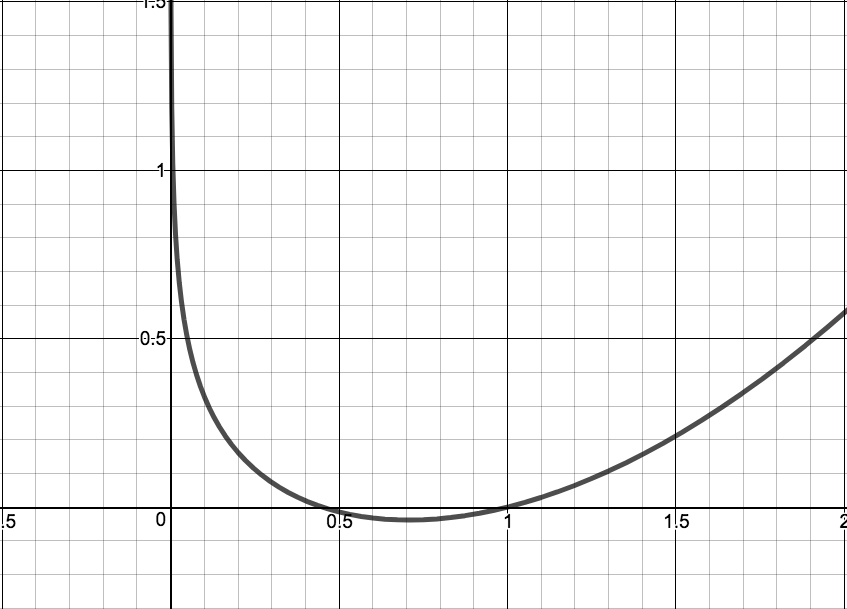
\includegraphics[height=1.5in]{./ApplicationsofExponentialandLogarithmicFunctionsGraphics/PURSUIT03.jpg}

\smallskip

$y(x) = \frac{1}{4} x^2-\frac{1}{4} \ln(x)-\frac{1}{4}$

\end{center}

\item The steady state current is 2 amps.

\addtocounter{enumi}{1}

\item  630 feet.

\item The linear regression on the data below is $y = 1.74899x + 0.70739$ with $r^{2} \approx 0.999995$.  

This is an excellent fit.

\scriptsize

\noindent \begin{tabular}{|l|r|r|r|r|r|r|r|r|r|r|} \hline
$x$ & 1 & 2 & 3 & 4 & 5 & 6 & 7 & 8 & 9 & 10 \\ 
\hline 
$\ln(N(x))$ & 2.4849 & 4.1897 & 5.9454 & 7.6967 & 9.4478 & 11.1988 & 12.9497 & 14.7006 & 16.4523 & 18.2025 \\ \hline
\end{tabular}

\normalsize

$N(x) = 2.02869(5.74879)^{x} = 2.02869e^{1.74899x}$ with $r^{2} \approx 0.999995$.  This is also an excellent fit and corresponds to our linearized model because $\ln(2.02869) \approx 0.70739$.

\item  \begin{enumerate}
\addtocounter{enumii}{1}

\item  The linearized model is: $\ln(L(x)) \approx 2.106 \ln(x) - 5.268$ with an $r^2 \approx  0.9914$.

\item  $L(x) = 0.005154 x^{2.106}$.  $L(90) \approx 67.3$ meaning the bottom $90 \%$ of wage earners take home $67.3 \%$ of the total national income.  Said differently, according to this model, the top $10 \%$ of wage earners take home $32.7 \%$ of the total national income. 



\item  We graph our answer to Example \ref{LorenzEx} in Section \ref{PowerFunctions}, $L(x) = 0.00027901x^{2.7738}$, below on the left.  Below on the right is the model we derived in this exercise. 

\begin{center}

\begin{tabular}{cc}

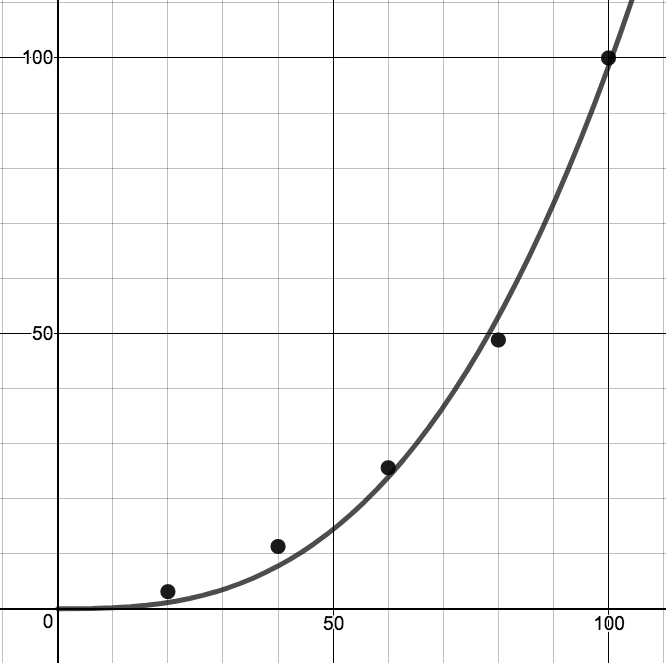
\includegraphics[height=1.5in]{./ApplicationsofExponentialandLogarithmicFunctionsGraphics/OldLorenzModel.jpg}  &

\hspace{1in}

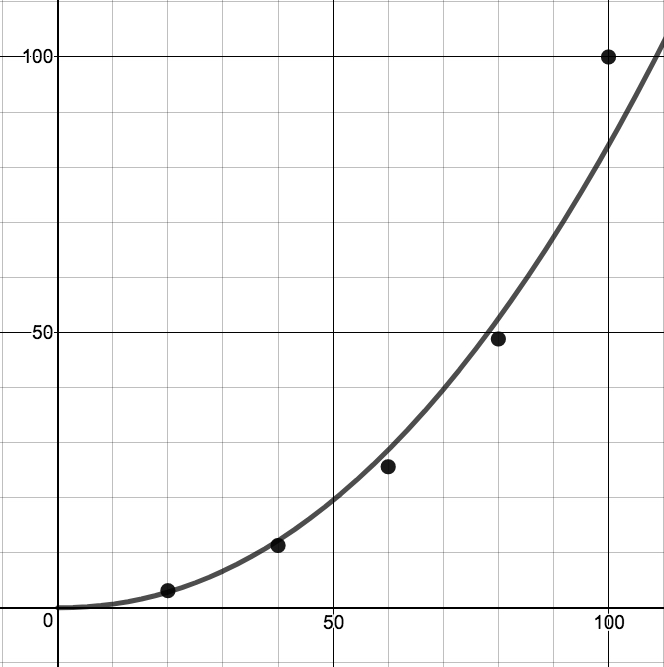
\includegraphics[height=1.5in]{./ApplicationsofExponentialandLogarithmicFunctionsGraphics/NewLorenzModel.jpg}  \\

 $L(x) = 0.00027901x^{2.7738}$

&

\hspace{1in}
$L(x) = 0.005154 x^{2.106}$ \\

\end{tabular}

\end{center}

\end{enumerate}


\item  \begin{enumerate}  \item   We get:  $y = 2895.06 (1.0147)^{x}$.  Graphing this along with our answer from Exercise \ref{PainesvillePopulationTwoPoint} over the interval $[0,60]$ shows that they are pretty close. From this model, $y(150) \approx 25840$ which once again overshoots the actual data value.

\item $P(150) \approx 18717$, so this model predicts 17,914 people in Painesville in 2010, a more conservative number than was recorded in the 2010 census.  We have $\ds{\lim_{t \rightarrow \infty} P(t) =  18691}$,  so the limiting population of Painesville based on this model is 18,691 people.

\enlargethispage{\baselineskip}

\end{enumerate}

\item \begin{enumerate}  \item  $y = \dfrac{242526}{1+874.63e^{-0.07113x}}$, where $x$ is the number of years since 1860.

\item  The plot of the data and the curve is below.

\centerline{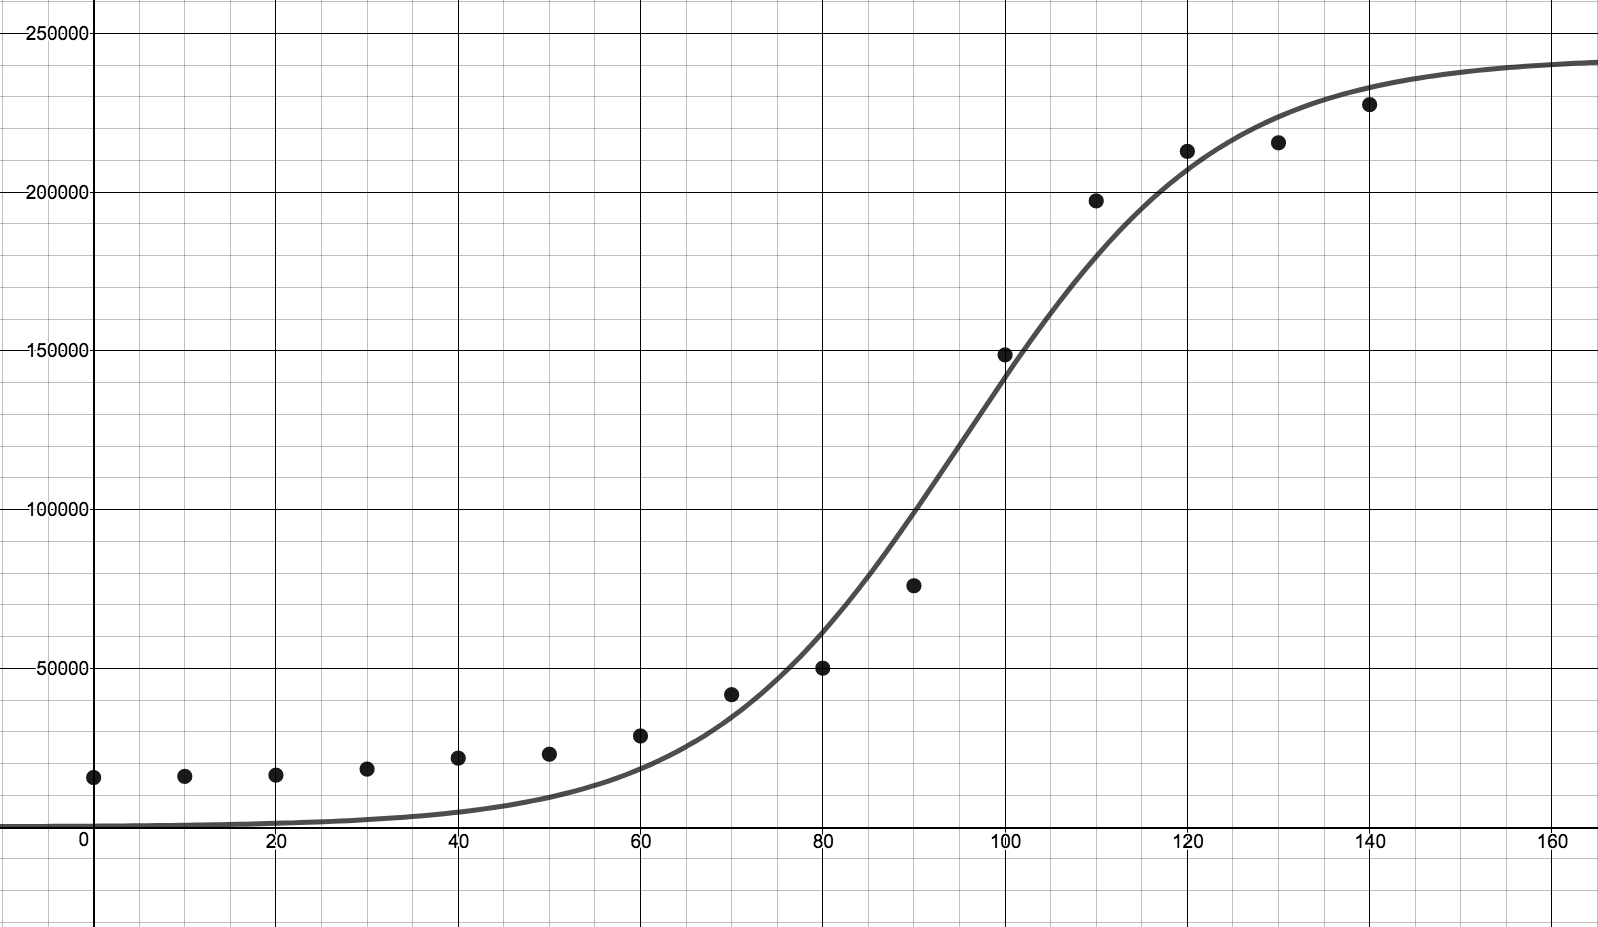
\includegraphics[height=2in]{./ApplicationsofExponentialandLogarithmicFunctionsGraphics/LAKECOUNTYLOGISTIC.jpg}} 

\item  $y(140) \approx 232884$, so this model predicts 232,884 people in Lake County in 2010.

\item  We get $\ds{\lim_{x \rightarrow \infty} y = 242526}$, so the limiting population of Lake County based on this model is 242,526 people.

\end{enumerate}

\end{enumerate}


\end{document}
